% ============================================================
% PRN232 - Section 5: Web Frontend (Vietnamese & English)
% ============================================================
\section{\bi{Cổng web Next.js 15}{The Next.js 15 Web Portal}}
\label{sec:web}

\subsection{\bi{Kiến trúc App Router}{App Router Architecture}}

\bi{
Cổng web được xây dựng bằng Next.js 15 với App Router, trên nền tảng
React 19 và Tailwind CSS với chủ đề ``Cinema Dark''. Kiến trúc App
Router thay thế mô hình \texttt{pages/} bằng cơ chế \emph{Server
Component} lồng nhau và \emph{Server Action}, cho phép dữ liệu được
lấy trực tiếp trên máy chủ mà không cần lớp API trung gian.
}{
The portal is built on Next.js 15 with the App Router, React 19 and
Tailwind CSS with a ``Cinema Dark'' theme. The App Router replaces the
\texttt{pages/} model with nested \emph{Server Components} and
\emph{Server Actions}, allowing data to be fetched directly on the
server without an intermediate API layer.
}

\begin{figure}[t]
\centering
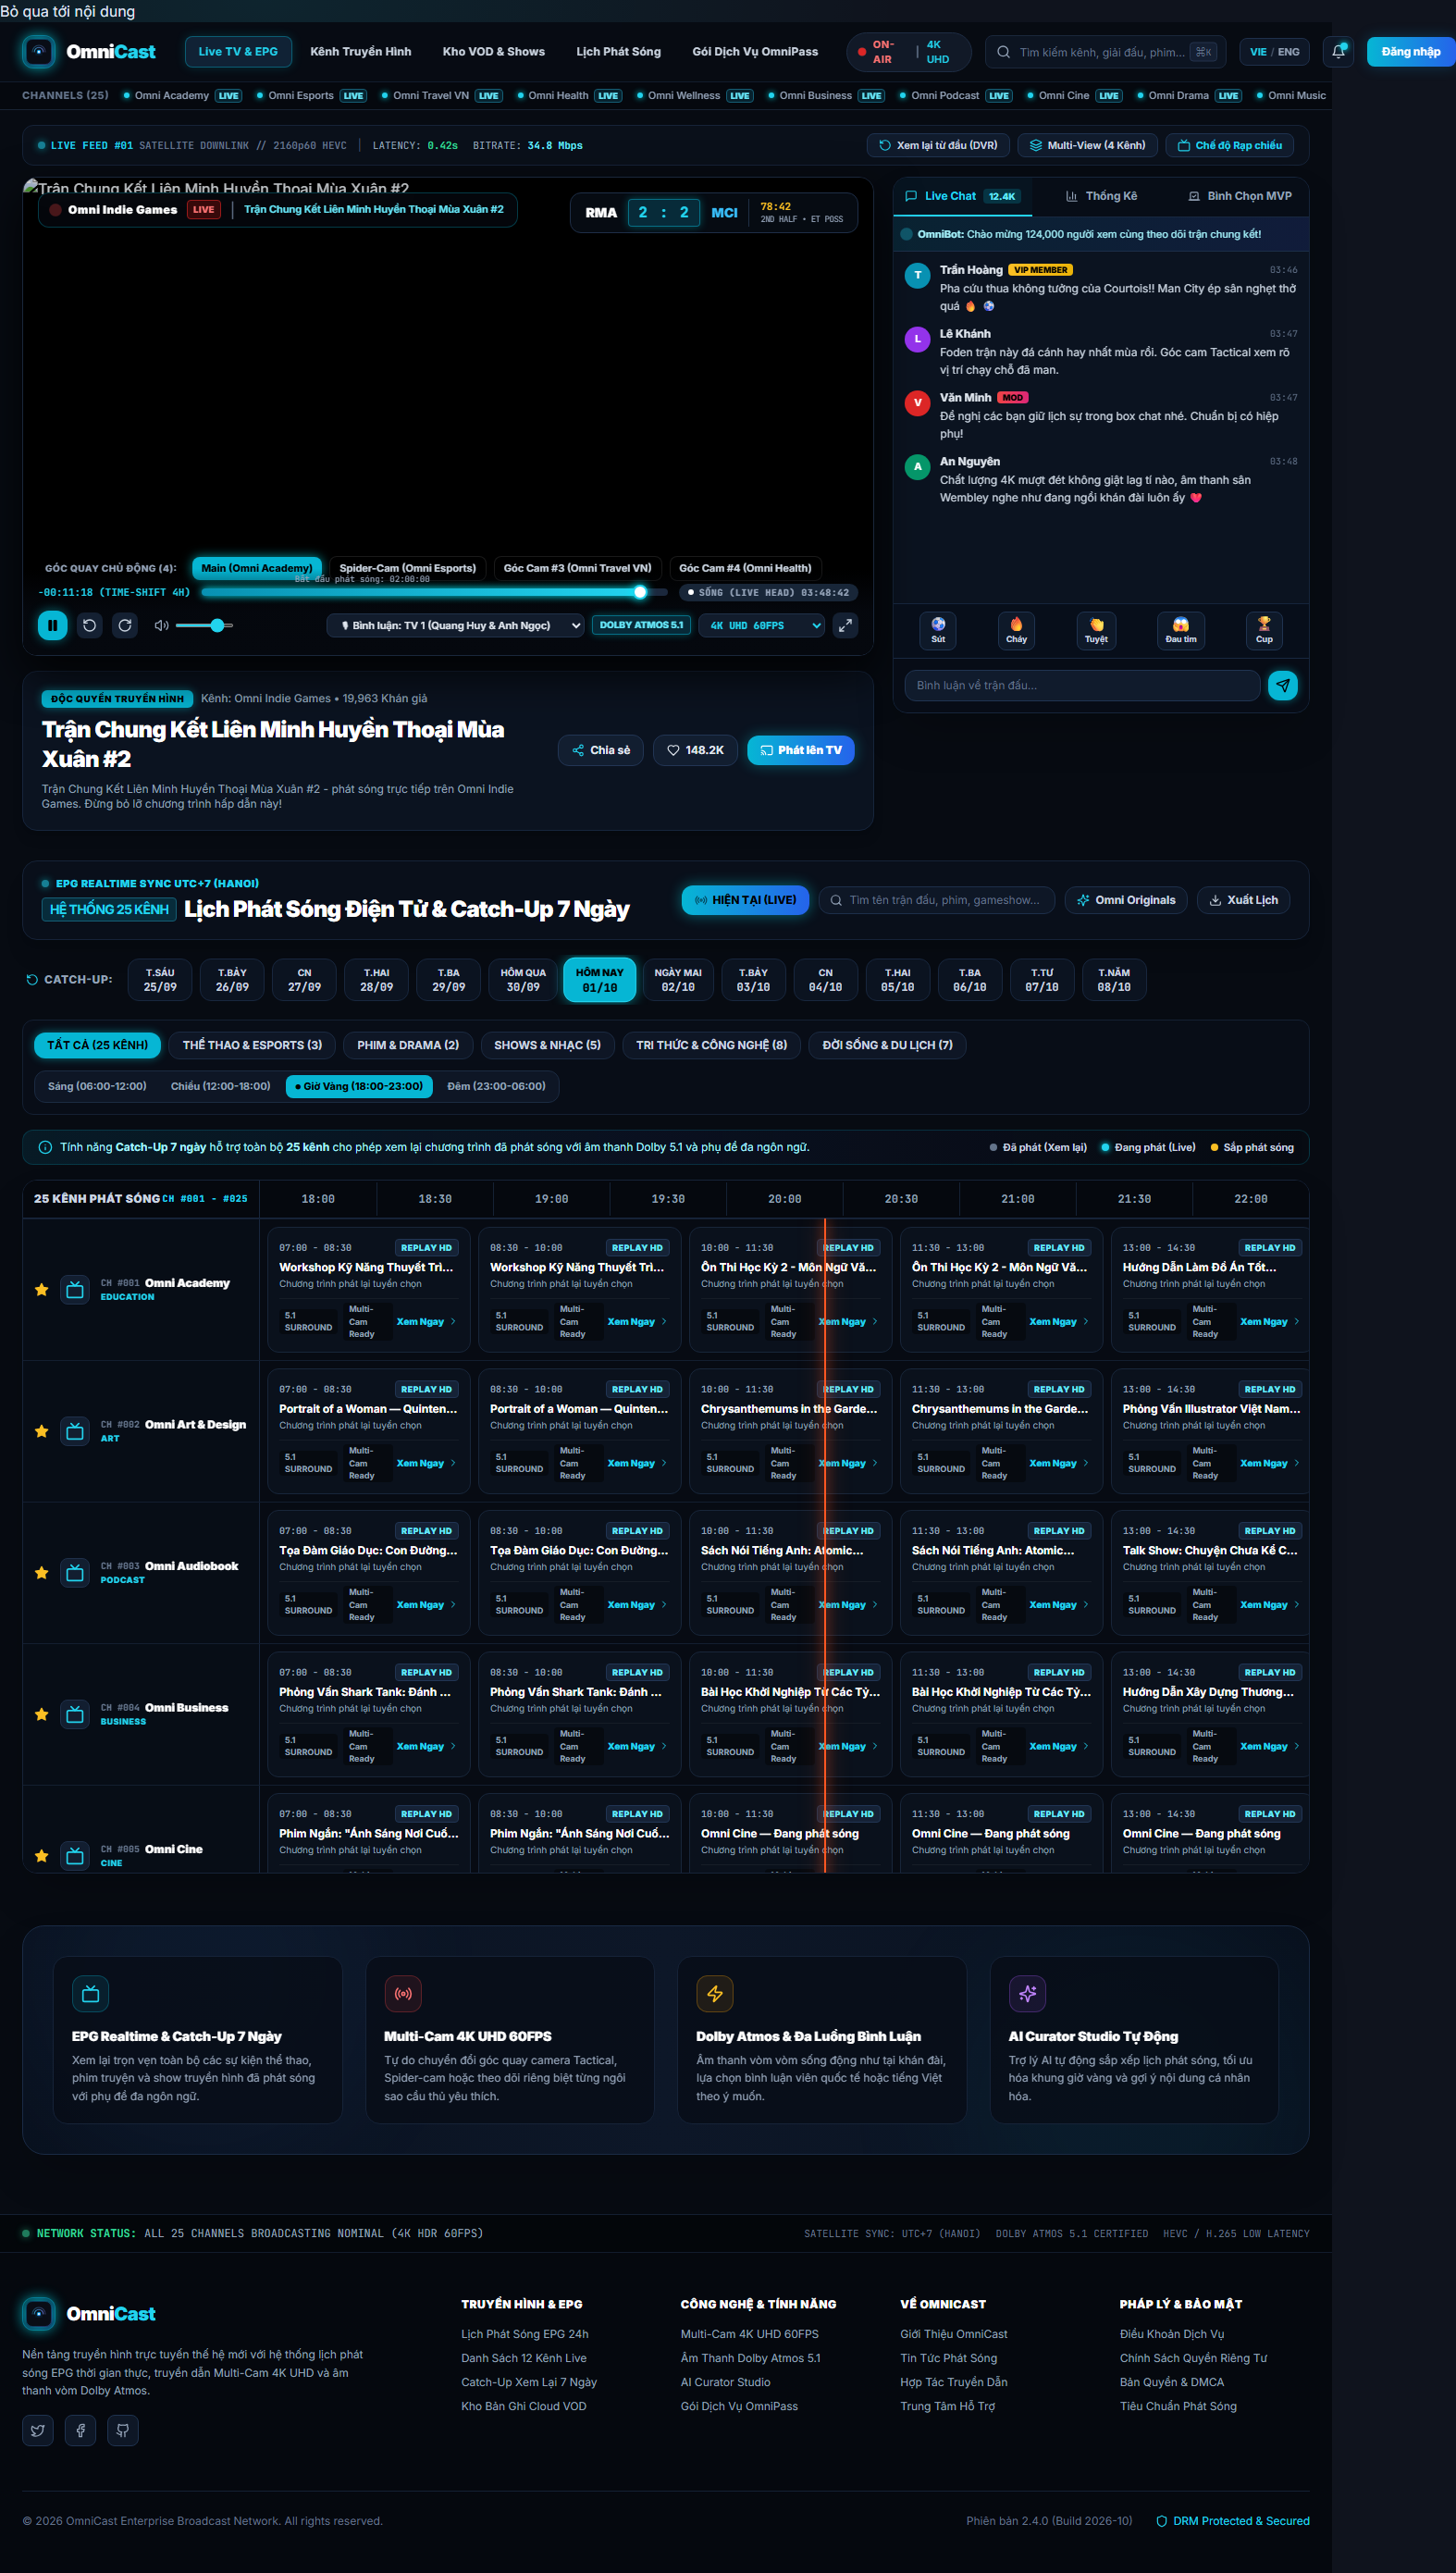
\includegraphics[width=\columnwidth]{../figures/01_home_desktop.png}
\caption{\bi{Trang chủ cổng web trên máy tính: carousel nổi bật, lưới
kênh theo thể loại và thanh điều hướng theo vai trò.}{The web portal
home page on desktop: featured carousel, channel grid by category and
the role-aware navigation bar.}}
\label{fig:home}
\end{figure}

\subsection{\bi{Danh mục đầy đủ 33 Route và Màn hình Web}{Complete 33-Route Web Portal Inventory}}

\bi{
Cổng web cung cấp đầy đủ 33 route được sinh từ 24 thư mục trong \texttt{frontend/app/}.
Bảng~\ref{tab:web_routes} liệt kê toàn bộ 33 màn hình được phân thành năm cụm chức năng:
(1) Nội dung \& Khám phá công khai; (2) Phòng xem LiveStream \& VOD; (3) Bàn điều khiển Live Studio \& Trợ lý AI Curator (\texttt{STAFF}/\texttt{ADMIN}); (4) Tài khoản, Cá nhân hoá \& Quản trị (\texttt{ADMIN}); và (5) Hệ thống Trang Pháp lý \& Tiêu chuẩn Phát sóng.
}{
The web portal exposes 33 routes generated from 24 directories under
\texttt{frontend/app/}. Table~\ref{tab:web_routes} catalogues all 33 screens across five functional clusters:
(1) Public Discovery \& EPG; (2) Interactive LiveStream \& VOD Rooms; (3) Live Studio Console \& AI Curator Suite (\texttt{STAFF}/\texttt{ADMIN}); (4) Account, Personalisation \& Administration (\texttt{ADMIN}); and (5) Legal, Compliance \& Broadcast Standards.
}

\begin{table*}[t]
\caption{\bi{Danh mục toàn bộ 33 Route và Màn hình trên Cổng Web Next.js 15 của OmniCast.}{Complete inventory of all 33 Next.js 15 web portal routes and screens in OmniCast.}}
\label{tab:web_routes}
\centering
\scriptsize
\begin{tabular}{@{}p{2.8cm}p{3.6cm}p{1.6cm}p{8.8cm}@{}}
\toprule
\textbf{\bi{Cụm chức năng}{Cluster}} & \textbf{\bi{Đường dẫn Route (33)}{Route Path (33)}} & \textbf{\bi{Phân quyền}{RBAC Role}} & \textbf{\bi{Tính năng \& Thao tác màn hình chính}{Key Screen Features \& Interactive Operations}} \\
\midrule
\multirow{6}{2.8cm}{\textbf{\bi{1. Khám phá \& Lịch phát EPG}{1. Public Discovery \& EPG}}}
  & \texttt{/}, \texttt{/channels}, \texttt{/channels/[id]} & Public & \bi{Carousel sự kiện tâm điểm, danh mục kênh lọc theo thể loại, trang chi tiết kênh kèm luồng đang phát \& lịch EPG.}{Hero spotlight carousel, category-filtered channel grid, channel detail page with live stream \& EPG.} \\
  & \texttt{/epg} & Public & \bi{Lưới lịch phát điện tử 24/7 không trống, thanh chỉ báo giờ hiện tại (Now-Line), lọc theo ngày và kênh.}{Zero-gap 24/7 EPG timeline grid, real-time Now-Line indicator, date and channel filters.} \\
  & \texttt{/programs}, \texttt{/programs/[id]} & Public & \bi{Thư viện chương trình, trang chi tiết chương trình kèm thẻ sản xuất, lịch phát sắp tới và nút lưu Watchlist.}{Programme directory, programme detail page with production tags, upcoming airings and Watchlist button.} \\
  & \texttt{/recordings}, \texttt{/recordings/[id]} & Public & \bi{Kho video VOD đã phát sóng, trình phát lại đa luồng kèm bình luận và gợi ý nội dung cùng thể loại.}{Published VOD recording library, multi-engine replay player with comments and related VODs.} \\
  & \texttt{/search} & Public & \bi{Tìm kiếm liên thực thể (Kênh, Chương trình, Bản ghi VOD) theo từ khóa và thể loại.}{Cross-entity search (Channels, Programmes, VOD Recordings) with keyword and genre filters.} \\
\midrule
\multirow{3}{2.8cm}{\textbf{\bi{2. Phòng Xem LiveStream}{2. LiveStream Rooms}}}
  & \texttt{/live} & Public & \bi{Trung tâm Đang Phát Sóng (Live Hub): tự động làm mới mỗi 15 giây, hiển thị tổng sự kiện LIVE \& tổng mắt xem (CCU), sắp xếp theo độ nóng hoặc mới nhất.}{Live Hub: auto-refreshes every 15s, displays active LIVE event \& total CCU pills, sorts by trending viewers or newest start time.} \\
  & \texttt{/live/[id]} & Public / Viewer & \bi{Phòng xem LiveStream tương tác: 7 giao diện chủ đề theo thể loại, Sảnh chờ \texttt{JoinLobbyCard}, Chế độ Rạp phim (Cinema Mode), đổi chương trình trong \texttt{lineup}, Chat thời gian thực, 4 nút Biểu cảm hạt nổi 0ms, Thông báo ghim từ Host.}{Interactive LiveStream Room: 7 genre-themed lounges, \texttt{JoinLobbyCard} prompt, Cinema Mode, lineup program switcher, real-time Socket.IO chat, 4 floating emoji reactions, pinned host banner.} \\
\midrule
\multirow{5}{2.8cm}{\textbf{\bi{3. Bàn điều khiển Live Studio \& AI}{3. Live Studio \& AI Curator}}}
  & \texttt{/studio}, \texttt{/studio/live} & \texttt{STAFF}+ & \bi{Bàn điều khiển phát sóng trực tiếp 4 Tab: (1) Chọn VOD có sẵn; (2) Tự ghi hình Camera/Màn hình WHIP WebRTC \& Upload kéo-thả có chữ ký Cloudinary; (3) Kho nội dung công khai; (4) Gửi thông báo ghim \& Dừng sóng.}{4-Tab Live Broadcast Console: (1) Curated VOD Live; (2) Camera/Screen WHIP WebRTC \& Signed Cloudinary Dropzone; (3) Verified Public Catalog; (4) Host Announcement \& Stop Broadcast.} \\
  & \texttt{/studio/curator} & \texttt{STAFF}+ & \bi{Trợ lý biên tập AI (\texttt{gpt-4o} + fallback heuristic): chấm điểm cảm xúc, kiểm duyệt đạo đức phát sóng, gợi ý thẻ và thể loại.}{AI Editorial Workbench (\texttt{gpt-4o} + heuristic fallback): sentiment scoring, broadcast compliance check, auto-tagging.} \\
  & \texttt{/studio/curator/audit}, \texttt{/studio/curator/dashboard} & \texttt{STAFF}+ & \bi{Nhật ký kiểm toán phiên bản prompt (\texttt{promptVersion}), thống kê tỷ lệ duyệt và hiệu năng gọi mô hình.}{Prompt-version provenance audit log (\texttt{promptVersion}), suitability breakdown and latency analytics.} \\
\midrule
\multirow{5}{2.8cm}{\textbf{\bi{4. Tài khoản, Cá nhân \& Quản trị}{4. Account \& Admin}}}
  & \texttt{/login}, \texttt{/register}, \texttt{/forgot-password}, \texttt{/reset-password} & Public & \bi{Đăng nhập JWT + Google OAuth2, đăng ký tài khoản, khôi phục mật khẩu qua mã xác thực.}{JWT + Google OAuth2 sign-in, account registration, tokenised password recovery.} \\
  & \texttt{/profile}, \texttt{/settings}, \texttt{/watchlist}, \texttt{/notifications} & \texttt{VIEWER}+ & \bi{Hồ sơ cá nhân, quản lý gói VIP, danh sách xem sau đồng bộ đa thiết bị, trung tâm thông báo và thu hồi phiên (\texttt{logout-all}).}{User profile, VIP plan management, cross-device watchlist, notification centre and global session revocation (\texttt{logout-all}).} \\
  & \texttt{/admin}, \texttt{/admin/users}, \texttt{/admin/audit-logs} & \texttt{ADMIN} & \bi{Tổng quan hệ thống, quản lý phân quyền người dùng, tra cứu nhật ký kiểm toán gRPC theo hành động/thực thể.}{System telemetry overview, user RBAC management, gRPC audit log explorer by action/entity.} \\
\midrule
\multirow{2}{2.8cm}{\textbf{\bi{5. Pháp lý \& Hỗ trợ}{5. Legal \& Support}}}
  & \texttt{/terms}, \texttt{/privacy}, \texttt{/dmca}, \texttt{/standards}, \texttt{/broadcasting-standards}, \texttt{/help}, \texttt{/docs} & Public & \bi{Điều khoản sử dụng, chính sách bảo mật, bản quyền DMCA, tiêu chuẩn cộng đồng \& phát sóng, trung tâm trợ giúp và tài liệu kỹ thuật.}{Terms of service, privacy policy, DMCA copyright policy, community \& broadcasting standards, help centre and docs.} \\
\bottomrule
\end{tabular}
\end{table*}

\begin{figure}[t]
\centering
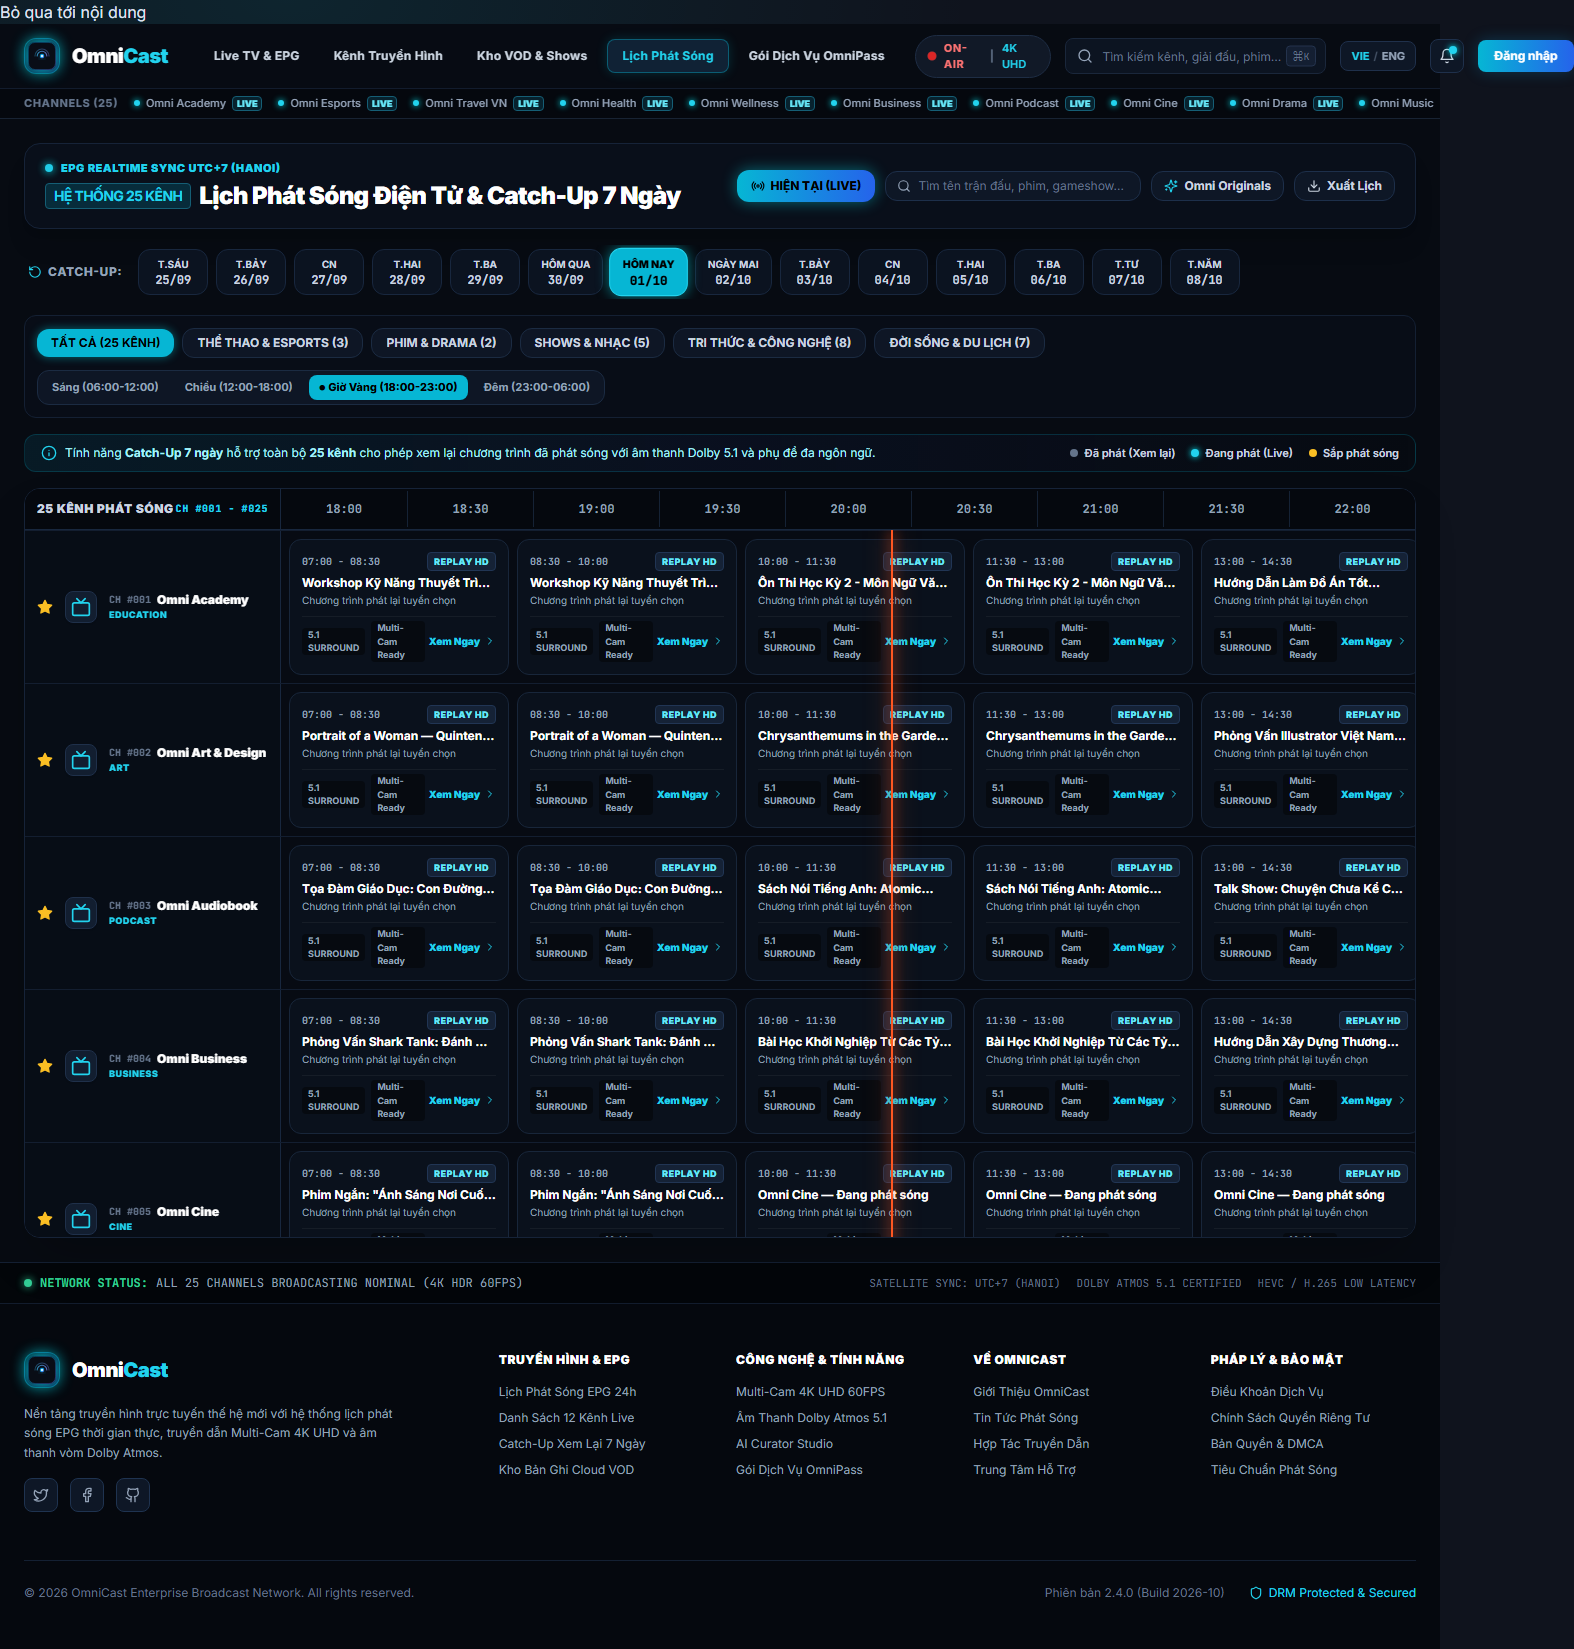
\includegraphics[width=\columnwidth]{../figures/subpage_epg.png}
\caption{\bi{Trang lịch phát điện tử (\texttt{/epg}) với lưới theo khung giờ và bộ chọn
ngày.}{The electronic programme guide page (\texttt{/epg}) with the time-slot grid and
the day selector.}}
\label{fig:epg}
\end{figure}

\subsection{\bi{Màn hình Phòng Xem LiveStream (\texttt{/live} \& \texttt{/live/[id]}) và Các Thao tác Tương tác}{Interactive LiveStream Room (\texttt{/live} \& \texttt{/live/[id]}) and Viewer Operations}}

\bi{
Hệ thống LiveStream trên Web được thiết kế như một không gian truyền hình tương tác toàn diện thông qua hai màn hình cốt lõi:
\begin{enumerate}[leftmargin=*,itemsep=2pt]
  \item \textbf{Trung tâm Phát sóng Trực tiếp (\texttt{/live}):} Tự động đồng bộ danh sách sự kiện đang \texttt{LIVE} mỗi 15 giây, hiển thị hai huy hiệu thống kê thời gian thực ở đầu trang (tổng số sự kiện đang phát và tổng số người đang xem đồng thời), hỗ trợ lọc và sắp xếp theo lượng người xem cao nhất hoặc thời điểm bắt đầu mới nhất, đồng thời hiển thị nút truy cập nhanh vào \texttt{/studio/live} cho người dùng có quyền \texttt{STAFF}/\texttt{ADMIN}.
  \item \textbf{Sảnh chờ Tham gia \& 7 Chủ đề Phòng Live (\texttt{/live/[id]}):} Khi truy cập vào một buổi phát sóng, người xem được chào đón bởi thẻ sảnh chờ \texttt{JoinLobbyCard} hiển thị ảnh thu nhỏ, trạng thái sóng, số mắt xem hiện tại và nút ``Tham gia phòng xem''. Đặc biệt, hàm \texttt{resolveLiveRoomTheme} tự động biến đổi toàn bộ bảng màu nền, viền phát sáng và huy hiệu của phòng xem theo \textbf{7 chủ đề thể loại}: \emph{Kids Wonderland} (Thiếu nhi), \emph{Podcast \& Audiobook} (Ấm áp), \emph{Music Live Stage} (Sân khấu âm nhạc), \emph{Academy \& Tech} (Giáo dục/Khoa học), \emph{Sports Arena} (Đấu trường thể thao), \emph{Obsidian Theater} (Điện ảnh/Phim truyện) và \emph{Broadcast Lounge} (Mặc định).
  \item \textbf{Trình phát Đa luồng, Chế độ Rạp phim (Cinema Mode) \& Chuyển chương trình tức thời:} Trình phát \texttt{VideoPlayer} tự động nhận diện luồng WebRTC/HLS từ MediaMTX (\texttt{cookieCheck=1}), luồng trực tiếp Google Drive hoặc nhúng YouTube. Người xem có thể bật \emph{Chế độ Rạp phim (Cinema Mode)} để làm tối toàn bộ phần tử xung quanh và mở rộng khung hình lên 12 cột. Nếu sự kiện có danh sách phát nhiều phần (\texttt{lineup}) hoặc người dùng là \texttt{STAFF}/\texttt{ADMIN}, thanh chọn chương trình cho phép chuyển đổi video đang phát ngay lập tức cho toàn bộ phòng qua API \texttt{switchProgramOnLiveEvent} mà không cần tải lại trang.
  \item \textbf{Thao tác Tương tác Thời gian thực qua Socket.IO (\texttt{/live}):} Khung tương tác bên phải kết nối trực tiếp tới namespace \texttt{/live}, cho phép khán giả: (i) gửi bình luận trực tiếp có kiểm tra đăng nhập và tự động cuộn mượt; (ii) thả 4 loại biểu cảm nổi (\texttt{HEART} $\heartsuit$, \texttt{FIRE}, \texttt{CLAP}, \texttt{WOW}) bay lên trên khung hình video kèm bộ đếm cộng dồn tức thời; và (iii) nhận thông báo ghim (\texttt{broadcaster:message}) từ đạo diễn hiển thị nổi bật dưới dạng dải băng thông báo ở đầu màn hình.
\end{enumerate}
}{
The web LiveStream experience is engineered as a full-featured interactive broadcast lounge across two core screens:
\begin{enumerate}[leftmargin=*,itemsep=2pt]
  \item \textbf{Live Broadcast Hub (\texttt{/live}):} Polls active \texttt{LIVE} events every 15 seconds, displays real-time header badges for total active broadcasts and aggregate concurrent viewers (CCU), supports sorting by viewer count or start time, and surfaces a direct ``Go to Live Studio'' shortcut for \texttt{STAFF}/\texttt{ADMIN} users.
  \item \textbf{Interactive Lobby \& 7 Genre-Themed Broadcast Lounges (\texttt{/live/[id]}):} Upon entering a stream, viewers encounter a \texttt{JoinLobbyCard} previewing the stream status and live viewer count before entering the room. Once inside, \texttt{resolveLiveRoomTheme} dynamically styles the entire room into one of \textbf{7 genre-specific themes}: \emph{Kids Wonderland}, \emph{Podcast \& Audiobook}, \emph{Music Live Stage}, \emph{Academy \& Tech}, \emph{Sports Arena}, \emph{Obsidian Theater} (Cinema/Drama) and \emph{Broadcast Lounge} (Default).
  \item \textbf{Multi-Engine Player, Cinema Mode \& Instant Lineup Switching:} \texttt{VideoPlayer} seamlessly handles MediaMTX HLS/WebRTC streams (\texttt{cookieCheck=1}), direct Google Drive streams and YouTube embeds. Viewers can toggle \emph{Cinema Mode} (lights-off focus) to dim surrounding chrome and expand the stage to full width. When a broadcast contains multiple lineup items or is controlled by \texttt{STAFF}/\texttt{ADMIN}, the lineup bar triggers \texttt{switchProgramOnLiveEvent}, switching the active video stream for all viewers in the room without page reload.
  \item \textbf{Real-Time Socket.IO (\texttt{/live}) Operations:} The live interaction sidebar connects to the \texttt{/live} namespace, enabling viewers to: (i) post real-time chat messages with auto-scroll; (ii) fire 4 floating emoji reactions (\texttt{HEART}, \texttt{FIRE}, \texttt{CLAP}, \texttt{WOW}) that animate upward over the video canvas with optimistic counter updates; and (iii) receive pinned host announcements (\texttt{broadcaster:message}) rendered as a prominent banner across the stage.
\end{enumerate}
}

\subsection{\bi{Màn hình Bàn điều khiển Web Live Studio (\texttt{/studio/live})}{Web Live Studio Broadcast Console (\texttt{/studio/live})}}

\bi{
Trang \texttt{/studio/live} (\texttt{frontend/app/studio/live/page.tsx}) cung cấp bàn điều khiển phát sóng chuyên nghiệp dành cho \texttt{STAFF} và \texttt{ADMIN} với 4 chế độ vận hành:
\begin{itemize}[leftmargin=*,itemsep=1pt]
  \item \textbf{Tab 1 --- Chọn nội dung phát sóng (Curated Live):} Chọn kênh đích, nhập tiêu đề/mô tả phiên Live, tìm kiếm và chọn một hoặc nhiều bản ghi từ thư viện kênh hoặc kho chung để phát sóng liên tiếp (\texttt{lineup}).
  \item \textbf{Tab 2 --- Tự ghi hình / Tải tệp / Phát trực tiếp từ Camera (\texttt{WebcamLiveBroadcaster} \& \texttt{WebStudioViewfinder}):} Hỗ trợ quay trực tiếp từ Camera máy tính, chia sẻ màn hình (\texttt{getDisplayMedia}), phát trực tiếp độ trễ thấp qua giao thức WebRTC WHIP tới MediaMTX, hoặc kéo-thả tệp video vào \texttt{UploadDropzone} + \texttt{UploadQueue} (tải lên trực tiếp Cloudinary bằng chữ ký số, hiển thị thanh tiến trình, tốc độ MB/s, thời gian còn lại ETA, tự động trích xuất ảnh thu nhỏ bằng \texttt{canvas} và hỗ trợ 3 chế độ xuất bản: Phát ngay \texttt{IMMEDIATE}, Hẹn lịch \texttt{SCHEDULED} hoặc Lưu nháp \texttt{PRIVATE}).
  \item \textbf{Tab 3 --- Kho nội dung công khai (Verified Public Catalog):} Duyệt danh sách các luồng HLS/MP4 công khai đã kiểm định, lọc theo định dạng và nhập một chạm vào thư viện kênh.
  \item \textbf{Tab 4 --- Điều hành \& Tương tác trực tiếp:} Cho phép đạo diễn gửi thông báo ghim (\texttt{broadcaster:message}) tới mọi người xem trong phòng và kết thúc phiên phát sóng (\texttt{stopLiveEvent}) kèm tùy chọn giữ lại bản ghi làm VOD.
\end{itemize}
}{
The \texttt{/studio/live} route (\texttt{frontend/app/studio/live/page.tsx}) provides a production-grade broadcast control console for \texttt{STAFF} and \texttt{ADMIN} operators across four tabs:
\begin{itemize}[leftmargin=*,itemsep=1pt]
  \item \textbf{Tab 1 --- Curated Live:} Select the target channel, configure broadcast metadata, and pick one or more VOD recordings from the channel or global library to launch a multi-item \texttt{lineup}.
  \item \textbf{Tab 2 --- Self-Record / File Upload / Webcam WHIP Live (\texttt{WebcamLiveBroadcaster} \& \texttt{WebStudioViewfinder}):} Supports browser camera capture, screen sharing (\texttt{getDisplayMedia}), direct WebRTC WHIP publishing to MediaMTX, or drag-and-drop file ingestion via \texttt{UploadDropzone} + \texttt{UploadQueue} (signed direct-to-Cloudinary upload with live MB/s speed, ETA, automatic HTML5 \texttt{canvas} thumbnail extraction, and 3 visibility modes: \texttt{IMMEDIATE}, \texttt{SCHEDULED}, \texttt{PRIVATE}).
  \item \textbf{Tab 3 --- Verified Public Catalog:} Browse verified HLS/MP4 streams with format filters and one-click channel library import.
  \item \textbf{Tab 4 --- Live Host Console:} Send pinned broadcaster announcements (\texttt{broadcaster:message}) to all connected viewers and terminate active broadcasts (\texttt{stopLiveEvent}) with the \texttt{keepAsVod} archival option.
\end{itemize}
}

\subsection{\bi{Giao diện theo vai trò và Trợ lý AI Curator}{Role-Aware Interface and AI Curator Suite}}

\bi{
Một tệp cấu hình duy nhất, \texttt{frontend/lib/constants/role-config.ts},
quyết định thành phần nào xuất hiện cho từng vai trò. Hàm
\texttt{hasMinimumRole} so sánh thứ hạng vai trò, nên việc nâng một
quyền từ \texttt{VIEWER} lên \texttt{STAFF} chỉ là sửa một dòng.
Trang \texttt{/studio/curator} là giao diện biên tập AI: hiển thị danh
sách chương trình chờ duyệt, cho phép chạy lại quy trình AI, xem
điểm tin cậy, phân loại phù hợp phát sóng và các cảnh báo tuân thủ.
Trang \texttt{/studio/curator/audit} trình bày lịch sử các lần chạy
AI với dấu vết phiên bản prompt, và \texttt{/studio/curator/dashboard} tổng hợp thống kê
phân bố theo thể loại và mức độ phù hợp phát sóng.
}{
A single configuration file,
\texttt{frontend/lib/constants/role-config.ts}, determines which
components appear for each role. The \texttt{hasMinimumRole} helper
compares role ranks, so promoting a capability from \texttt{VIEWER} to
\texttt{STAFF} is a one-line edit. The \texttt{/studio/curator} page is the AI curation interface: it
lists programmes awaiting review, allows re-running the AI pipeline,
and exposes the confidence score, broadcast-suitability classification
and compliance flags. The \texttt{/studio/curator/audit} page presents
the run history with prompt-version provenance, while \texttt{/studio/curator/dashboard}
aggregates statistics by category and broadcast suitability.
}

\begin{figure}[t]
\centering
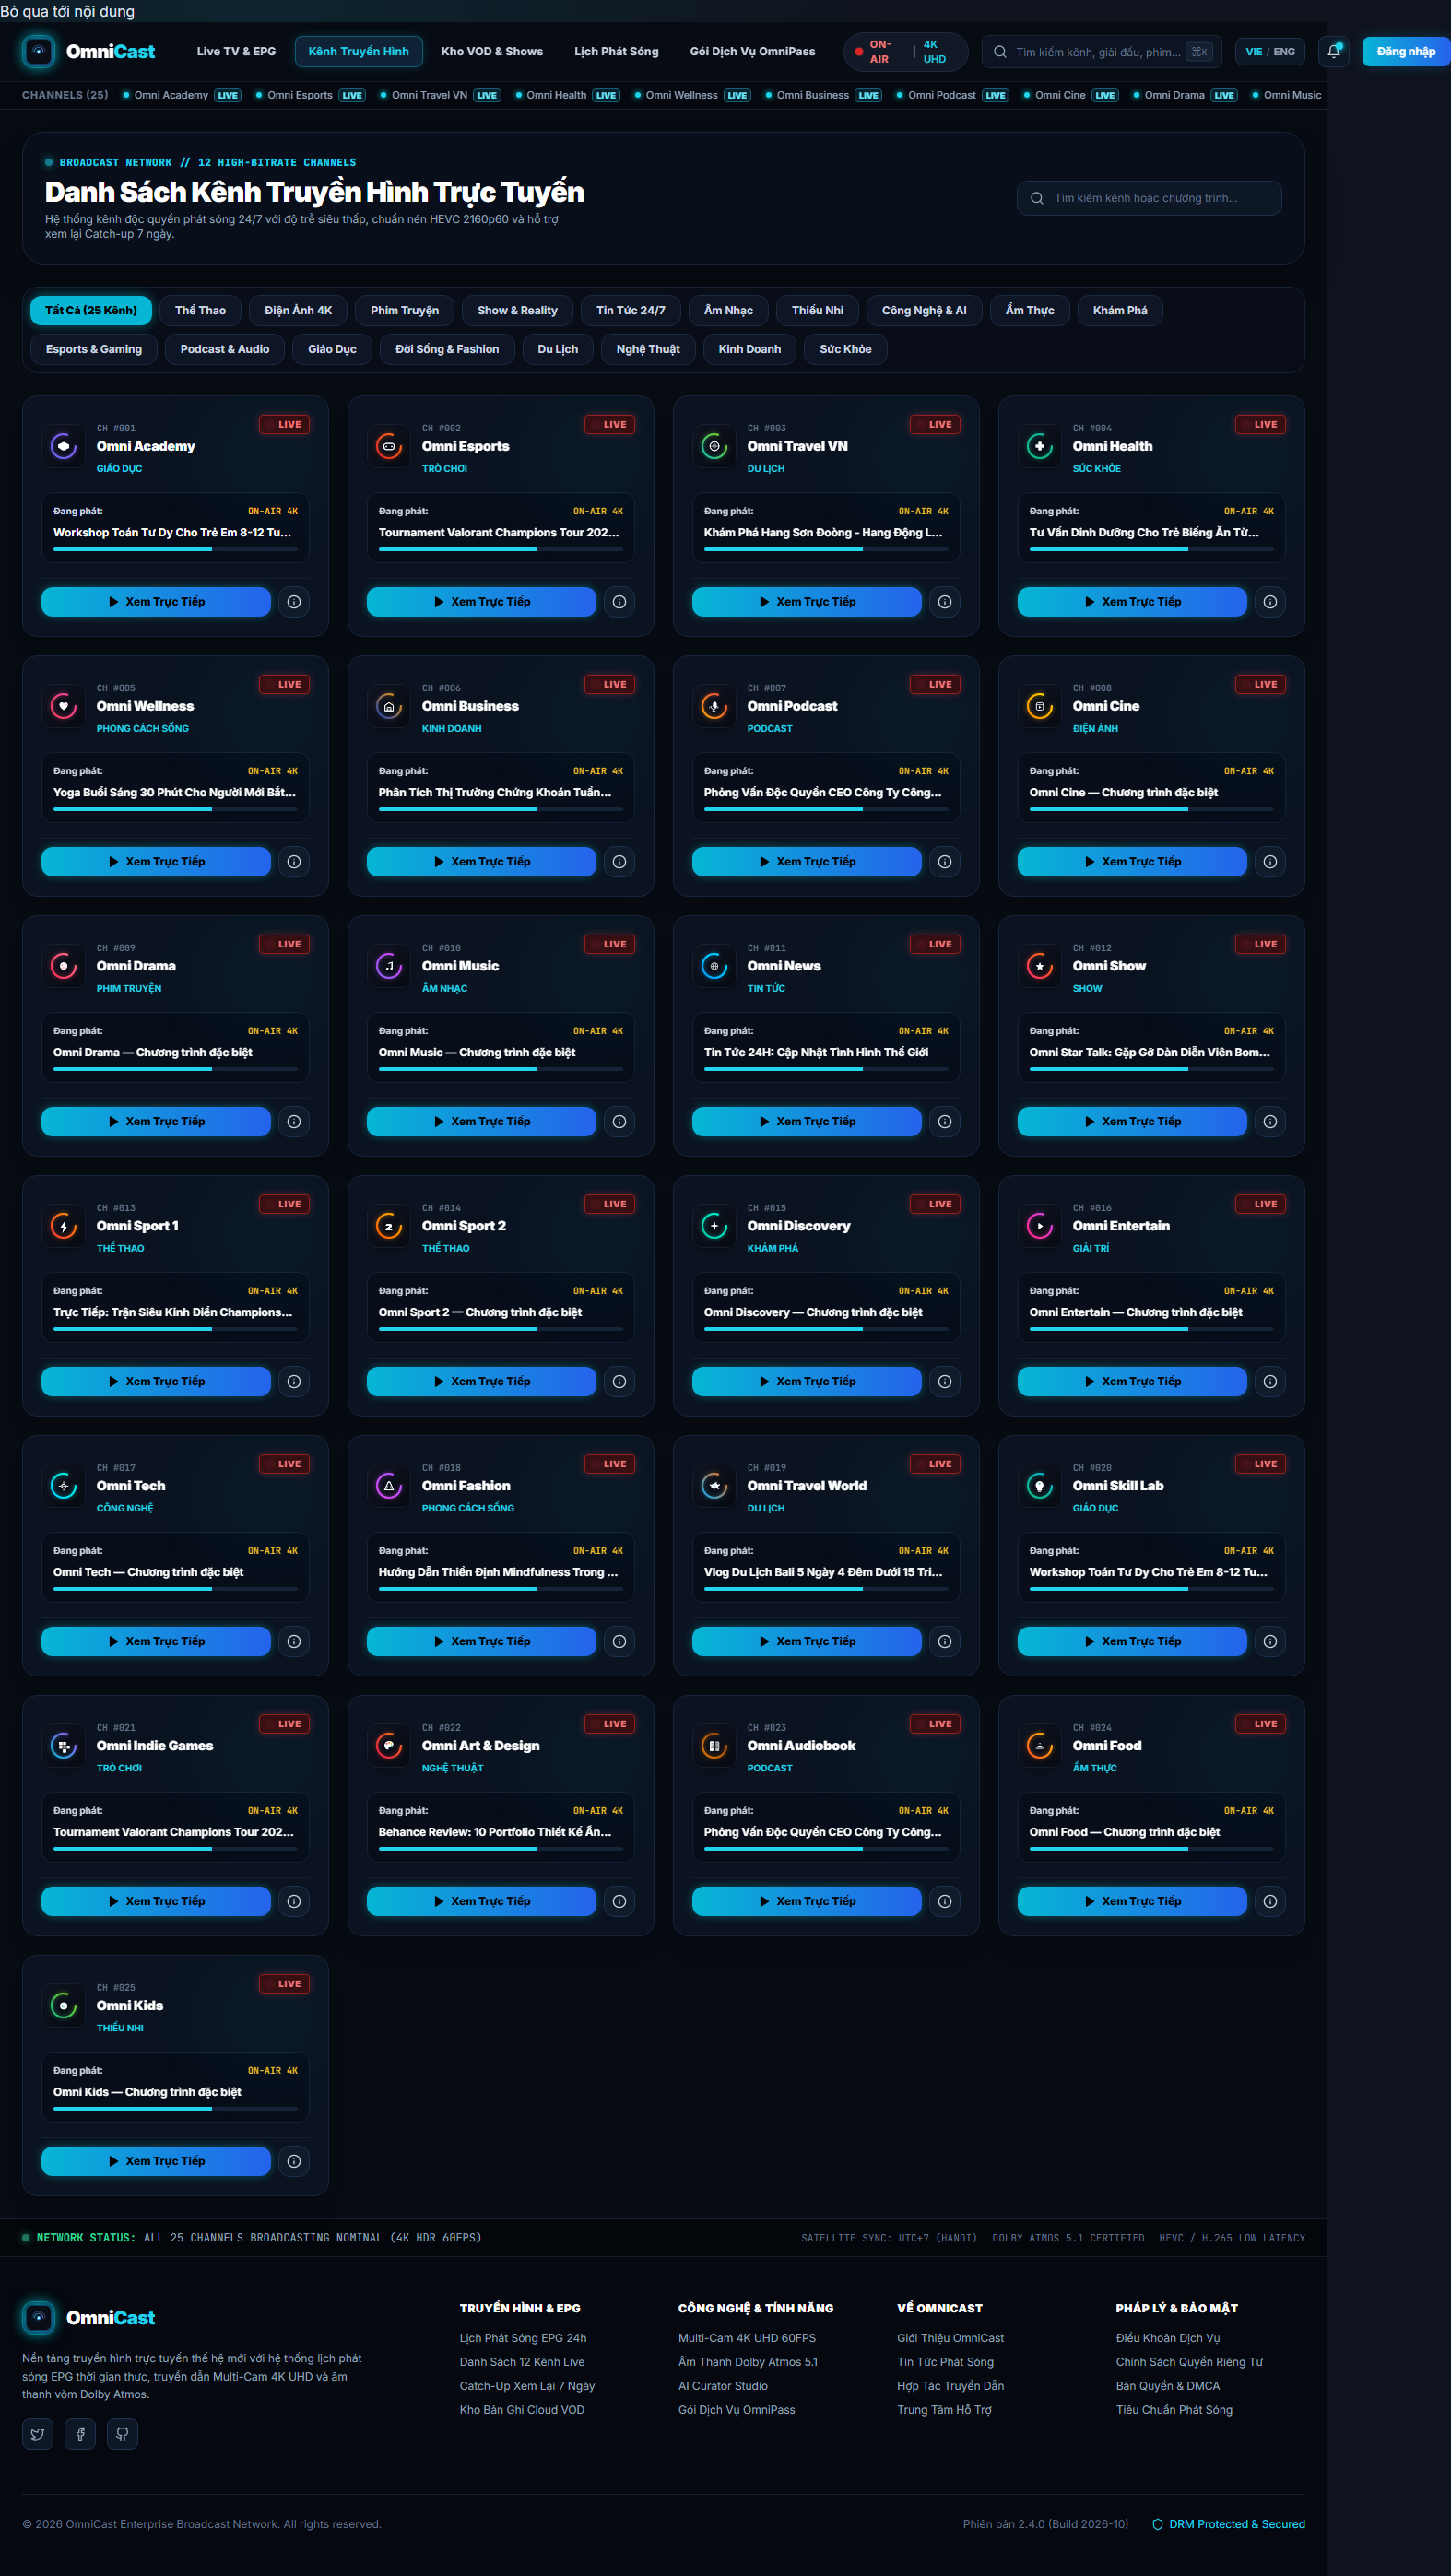
\includegraphics[width=\columnwidth]{../figures/subpage_channels.png}
\caption{\bi{Trang danh mục kênh (\texttt{/channels}) với bộ lọc theo thể loại và thẻ nội
dung.}{The channel catalogue page (\texttt{/channels}) with category filters and content
badges.}}
\label{fig:channels}
\end{figure}

\subsection{\bi{Bảo mật phía client, Quản lý phiên và Kiểm thử}{Client-Side Security, Session Handling and Testing}}

\bi{
Cổng web dùng \texttt{next-themes} để hỗ trợ chế độ sáng/tối và một
lớp \texttt{safe-log} (\texttt{redact.ts}) loại bỏ mọi dữ liệu nhạy cảm (mật khẩu, token, khóa API) trước khi ghi log. Khi người dùng đăng xuất, mọi phiên đăng nhập trên thiết bị khác được
thu hồi qua endpoint \texttt{logout-all}.
Cổng web có 228 kiểm thử Vitest trong 76 bộ kiểm thử, bao phủ các hàm
thuần (\texttt{query-builder}, \texttt{curator-filters},
\texttt{curator-helpers}, \texttt{redact}, \texttt{safe-log},
\texttt{utils}), các hook (\texttt{useAiCurator},
\texttt{useAiCuratorStats}), các hàm cấu hình (\texttt{role-config}) và
các thành phần React (\texttt{video-player},
\texttt{save-to-watchlist}, các trang pháp lý, các trang studio).
CI còn chạy \texttt{tsc --noEmit} để bắt lỗi kiểu dữ liệu trước khi
biên dịch.
}{
The portal uses \texttt{next-themes} for light/dark support and a
\texttt{safe-log} layer (\texttt{redact.ts}) that masks sensitive fields (passwords, tokens, API keys) before logging. On
logout, sessions on other devices are revoked through the
\texttt{logout-all} endpoint.
The portal carries 228 Vitest tests across 76 suites, covering pure
functions (\texttt{query-builder}, \texttt{curator-filters},
\texttt{curator-helpers}, \texttt{redact}, \texttt{safe-log},
\texttt{utils}), hooks (\texttt{useAiCurator},
\texttt{useAiCuratorStats}), configuration (\texttt{role-config}) and
React components (\texttt{video-player}, \texttt{save-to-watchlist},
the legal pages, the studio pages). CI additionally runs
\texttt{tsc --noEmit} to catch type errors before the build.
}
